\section{Supplementary fitted functions on the sphere}
\label{app:sphere-endpoints}

Figure~\ref{fig:sphere-orders} adds a three-dimensional-input, four-hidden-layer
example.  The sphere RMS discrepancies from dense are $0.02193$, $0.01280$,
and $0.00454$ for $P=1,2,3$.  Dense and the three closures reach training
RMS $\leq0.01$ at times $60$, $75.5$, $63.25$, and $60$, respectively.
This is supplementary fitted-function evidence outside the smooth-activation
theorems: ReLU is nonsmooth, and the endpoints are individually fitted.
Rendering the saved predictions does not independently reproduce training.

\begin{figure}[!htbp]
  \centering
  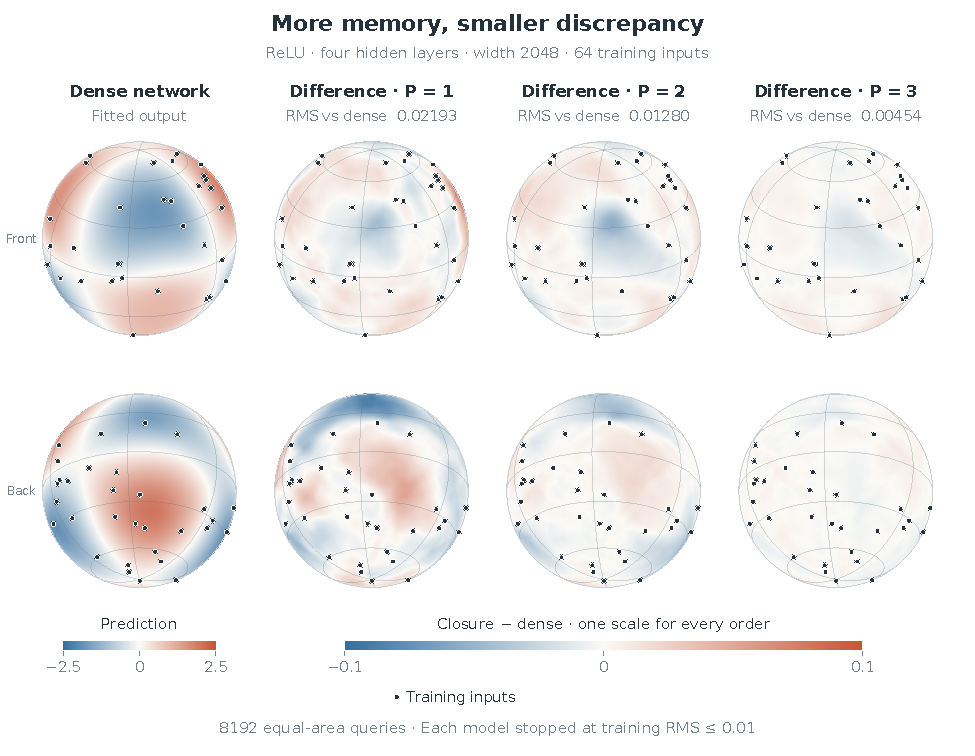
\includegraphics[width=\textwidth]{figures/sphere_orders.pdf}
  \caption{Saved fitted functions on the unit sphere for the target
  $\sqrt{105}\,x_1x_2x_3$, with four hidden ReLU layers of width $2048$ and
  $64$ training inputs.  The first column shows the dense output; the remaining
  columns show signed closure-minus-dense differences for $P=1,2,3$.
  Rows show complementary hemispheres, and black dots mark training inputs.
  Output colors use $[-2.5,2.5]$; every error panel uses $[-0.1,0.1]$.
  Surface colors interpolate saved queries on a triangular mesh; RMS values
  use the original $8192$ equal-area query values before interpolation.
  Models are compared at their individual training-RMS $\leq0.01$ endpoints,
  using one network seed and float32 Euler steps of $1/128$.
  The order trend is specific to this one-seed comparison.  These are
  fitted-function discrepancies, without a common-time trajectory comparison
  or a continuous-gradient-flow refinement certificate.}
  \label{fig:sphere-orders}
\end{figure}
